\begin{table}[H]
	\centering
	\caption{Blocking Probabilities (As given by Erlang-B Chart)}
	\label{tab:erlang}
	\begin{tabular}{|c|c|c|c|c|}
	\hline
	Number of Channels & Blocking Probability
		     & Initialisation Cost & Blocking Cost
		     & Total Cost \\
	(W) & (B) & (1.2 x W) & (3.1 x 10 x B) & (IC + BC)\\
	\hline
	4 & 0.6467    & 4.8  & 20.047 & 24.847		\\
	8 & 0.3383    & 9.6  & 10.488 & 20.088 		\\
	12 & 0.1197   & 14.4 & 3.712  & 18.119		\\
	16 & 0.0223   & 19.2 & 0.6914 & 19.891		\\
	20 & 0.0019   & 24   & 0.0589 & 24.058		\\
	\hline
	\end{tabular}
\end{table}

The following plot shows the total overall costs for between zero and 25
channels.

\begin{figure}[H]
	\centering
	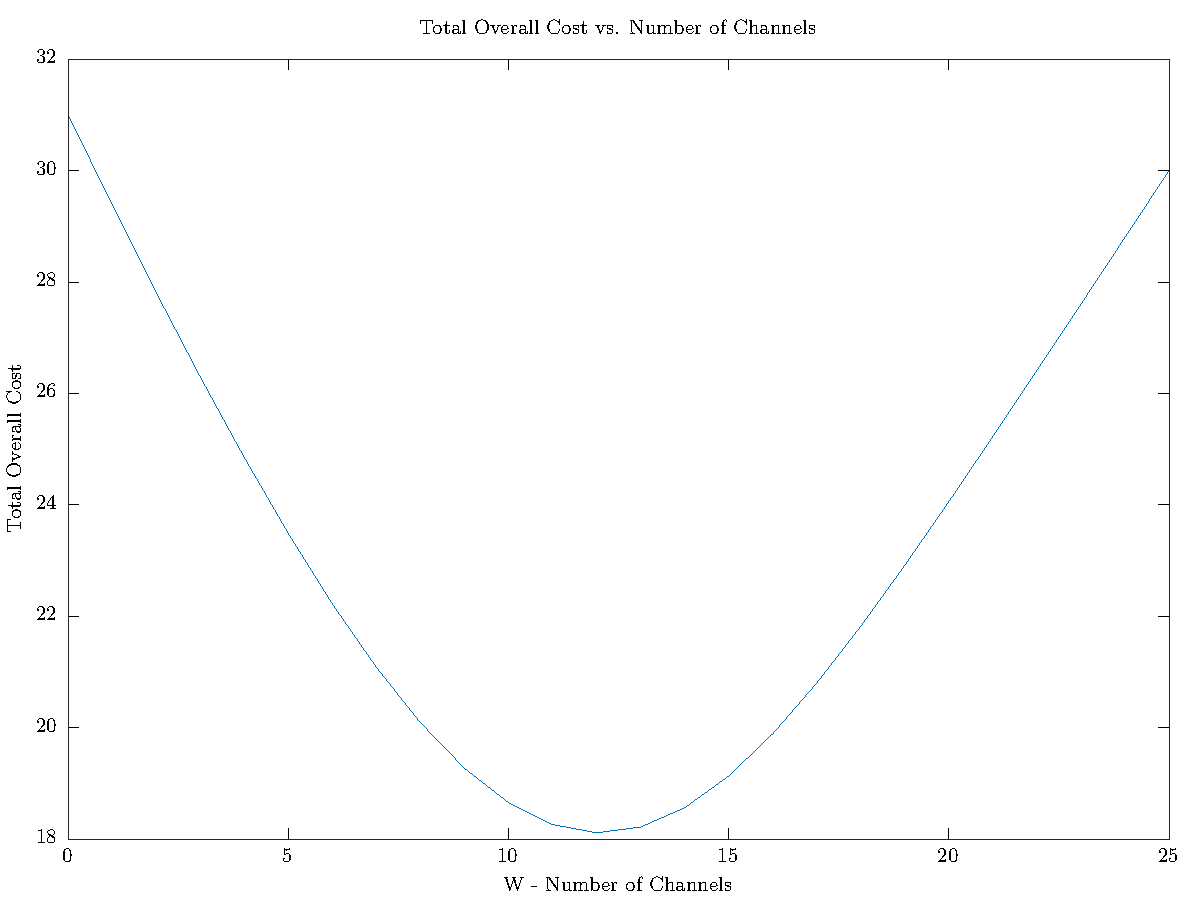
\includegraphics[width=0.8\textwidth]{code/Q5/Q5}
	\caption{Plot of the Total Overall Cost within the given system}
	\label{fig:code-Q5}
\end{figure}

Therefore, the number of channels which minimizes the total overall cost is 12.

The above answers were obtained using the Erlang-B Iterative Formula, programmed
using GNU-Octave. This code is shown below.

\lstinputlisting[language=Octave]{code/Q5/erlang.m}

